% Chapter 8: Sample Efficiency and Multi-Fidelity Optimization
% IEEE-Style Academic Textbook Chapter


\begin{abstract}
The optimization of synthetic data generation parameters for object detection models presents a fundamentally challenging sample efficiency problem. Each evaluation of a candidate parameter configuration requires generating synthetic images, training a deep neural network such as YOLO, and evaluating performance on real-world validation data. This computational pipeline renders traditional reinforcement learning approaches, which typically require millions of environment interactions, entirely impractical. This chapter develops a comprehensive framework for sample-efficient optimization in this expensive black-box setting, introducing multi-fidelity techniques, adaptive budget allocation strategies, and principled convergence detection methods that collectively enable effective optimization within strict computational constraints.
\end{abstract}

\section{The Sample Efficiency Challenge}
\label{sec:sample_efficiency_challenge}

The synthesis of training data for deep learning models through parametric generators introduces an optimization problem of considerable computational complexity. Unlike conventional hyperparameter tuning where model training represents the primary computational burden, synthetic data optimization compounds this cost with additional data generation overhead and the fundamental challenge of evaluating transfer performance from synthetic to real domains. Understanding the precise cost structure of this optimization problem is essential for designing algorithms that can achieve meaningful results within practical resource constraints.

\subsection{Cost Model for Synthetic Data Optimization}
\label{subsec:cost_model}

The total computational cost of evaluating a single configuration $\theta$ in the synthetic data optimization pipeline can be decomposed into three primary components. Let $C_{\text{gen}}(\theta, n)$ denote the cost of generating $n$ synthetic images with parameters $\theta$, $C_{\text{train}}(n, e)$ the cost of training the object detection model on $n$ images for $e$ epochs, and $C_{\text{eval}}$ the cost of evaluating the trained model on the real-world validation set. The total evaluation cost becomes:

\begin{equation}
C_{\text{total}}(\theta) = C_{\text{gen}}(\theta, n) + C_{\text{train}}(n, e) + C_{\text{eval}}
\label{eq:total_cost}
\end{equation}

For modern object detection architectures such as YOLOv8, training on a dataset of 5,000 synthetic images for 100 epochs on a contemporary GPU requires approximately 2-4 hours of wall-clock time. When multiplied across the hundreds of evaluations typically required for black-box optimization, the total computational budget can easily exceed thousands of GPU-hours. This cost structure fundamentally differentiates synthetic data optimization from conventional machine learning hyperparameter tuning, where individual evaluations may complete in minutes rather than hours.

The generation cost $C_{\text{gen}}(\theta, n)$ depends critically on the complexity of the synthetic data pipeline. Procedural generation systems based on domain randomization typically exhibit linear scaling with dataset size, while physics-based rendering engines may introduce substantial per-image overhead. For rendering engines such as BlenderProc or NVIDIA Isaac Sim, generating photorealistic synthetic images can require 1-10 seconds per image depending on scene complexity, material properties, and lighting configurations. A dataset of 5,000 images thus requires 1.5-14 hours of generation time, representing a non-negligible fraction of the total evaluation cost.

\subsection{Comparison with Traditional Reinforcement Learning}

Traditional deep reinforcement learning algorithms exhibit sample complexities that are fundamentally incompatible with the synthetic data optimization setting. Proximal Policy Optimization and similar policy gradient methods typically require $10^6$ to $10^9$ environment interactions to learn effective policies in continuous control tasks. Model-free approaches such as Deep Q-Networks demonstrate comparable sample requirements, with successful Atari game playing requiring approximately $10^8$ frames of experience.

The synthetic data optimization problem admits at most $10^2$ to $10^3$ evaluations within reasonable computational budgets, representing a gap of four to seven orders of magnitude relative to conventional reinforcement learning requirements. This disparity motivates the adoption of fundamentally different algorithmic approaches designed specifically for expensive black-box optimization. Bayesian optimization and its multi-fidelity extensions provide the theoretical foundation for achieving meaningful optimization progress within such severely constrained evaluation budgets.

Model-based reinforcement learning offers potential improvements in sample efficiency through the construction of learned dynamics models that enable policy optimization through simulated rollouts. World model approaches such as DreamerV3 have demonstrated the ability to learn complex behaviors with substantially reduced environment interactions, achieving near-optimal performance in some domains with as few as $5 \times 10^4$ interactions. However, even these improved sample complexities remain orders of magnitude beyond what the synthetic data optimization setting permits, necessitating further algorithmic innovations.

Figure~\ref{fig:sample_efficiency_comparison} illustrates the stark difference in sample requirements between traditional reinforcement learning approaches and the multi-fidelity methods developed in this chapter.

\begin{figure}[htbp]
\centering
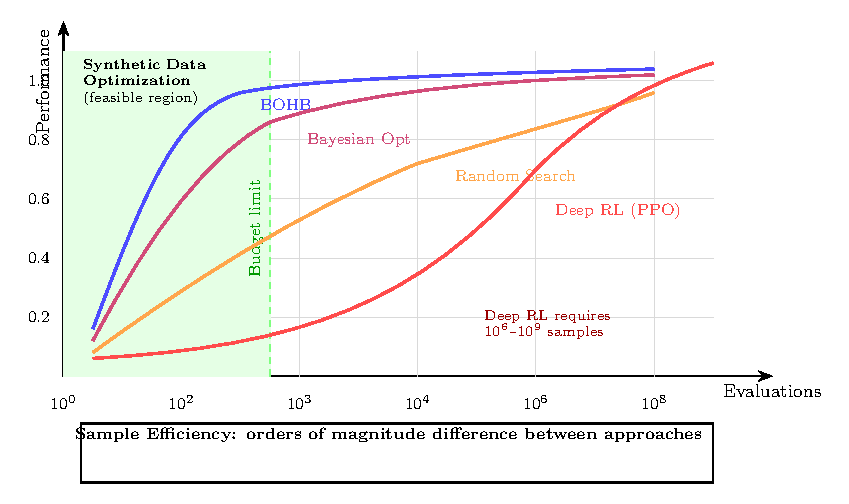
\includegraphics[width=0.85\textwidth]{figures/ch08_fig3_sample_efficiency.pdf}
\caption{Sample efficiency comparison across optimization approaches. Traditional deep reinforcement learning methods (e.g., PPO) require $10^6$--$10^9$ evaluations, far exceeding the feasible budget for synthetic data optimization. Multi-fidelity methods like BOHB achieve competitive performance within the practical budget limit of $10^2$--$10^3$ evaluations, representing a four to seven order-of-magnitude improvement in sample efficiency.}
\label{fig:sample_efficiency_comparison}
\end{figure}

\subsection{Budget Constraints in Practice}

Practical synthetic data optimization projects operate under multiple interacting constraints that collectively define the feasible optimization budget. Hardware availability determines the maximum parallelism achievable during evaluation, with typical academic and industrial settings providing access to 1-8 GPUs for sustained optimization campaigns. Project timelines impose wall-clock time limits that, combined with per-evaluation durations, bound the total number of sequential evaluations. Financial considerations in cloud computing environments translate directly to evaluation count limits through hourly GPU rental costs.

A representative budget for a synthetic data optimization project targeting industrial deployment might allocate 100-200 GPU-hours to the optimization process. With per-evaluation costs of 2-4 GPU-hours for full-fidelity training, this budget permits only 25-100 complete evaluations. The multi-fidelity techniques developed in subsequent sections enable more effective utilization of this limited budget by strategically allocating resources across evaluations of varying computational cost.

\section{Multi-Fidelity Optimization Framework}
\label{sec:multi_fidelity_framework}

Multi-fidelity optimization exploits the observation that expensive objective functions often admit cheaper approximations that correlate with the true objective. In the synthetic data optimization context, these approximations arise naturally through reduced training duration and smaller dataset sizes, both of which decrease computational cost while providing informative signals about configuration quality.

\subsection{Fidelity Dimensions}

The synthetic data optimization pipeline admits multiple independent dimensions along which fidelity can be varied. The training epoch dimension controls the number of complete passes through the training dataset, with early-epoch performance providing a noisy but correlated estimate of final performance. The dataset size dimension controls the number of synthetic images generated and used for training, with smaller datasets enabling faster generation and training at the cost of increased variance in the resulting model quality.

Formally, we extend the objective function to incorporate fidelity parameters:

\begin{equation}
f(\theta, r) : \Theta \times \mathcal{R} \rightarrow \mathbb{R}
\label{eq:multi_fidelity_objective}
\end{equation}

where $r = (r_{\text{epochs}}, r_{\text{data}}) \in \mathcal{R}$ represents the fidelity configuration and $\mathcal{R} = [r_{\min}^{\text{epochs}}, r_{\max}^{\text{epochs}}] \times [r_{\min}^{\text{data}}, r_{\max}^{\text{data}}]$ defines the fidelity space. The cost function $c(\theta, r)$ increases monotonically with both fidelity dimensions, while the correlation between $f(\theta, r)$ and the true objective $f(\theta, r_{\max})$ generally increases with fidelity.

\subsection{Fidelity Level Definitions}

Effective multi-fidelity optimization requires careful definition of discrete fidelity levels that balance computational cost against information quality. Table~\ref{tab:fidelity_levels} presents recommended fidelity configurations for synthetic data optimization with YOLO-family architectures, based on empirical observations of the cost-correlation tradeoff.

\begin{table}[htbp]
\centering
\caption{Multi-Fidelity Level Definitions for Synthetic Data Optimization}
\label{tab:fidelity_levels}
\begin{tabular}{lcccc}
\hline
\textbf{Fidelity Level} & \textbf{Epochs} & \textbf{Dataset Size} & \textbf{Relative Cost} & \textbf{Correlation} \\
\hline
Ultra-Low & 10 & 500 & 0.02 & 0.55--0.65 \\
Low & 25 & 1,000 & 0.08 & 0.70--0.80 \\
Medium & 50 & 2,500 & 0.25 & 0.85--0.90 \\
High & 100 & 5,000 & 1.00 & 1.00 \\
\hline
\end{tabular}
\end{table}

The correlation values in Table~\ref{tab:fidelity_levels} represent empirically observed rank correlations between configuration performance at each fidelity level and full-fidelity performance. These correlations exhibit substantial task dependence, with simpler detection problems showing higher correlations at lower fidelities while complex multi-class detection scenarios may require higher minimum fidelities for reliable configuration comparison.

Figure~\ref{fig:fidelity_pyramid} provides a visual representation of the multi-fidelity hierarchy, illustrating the tradeoff between computational cost and correlation with full-fidelity performance.

\begin{figure}[htbp]
\centering
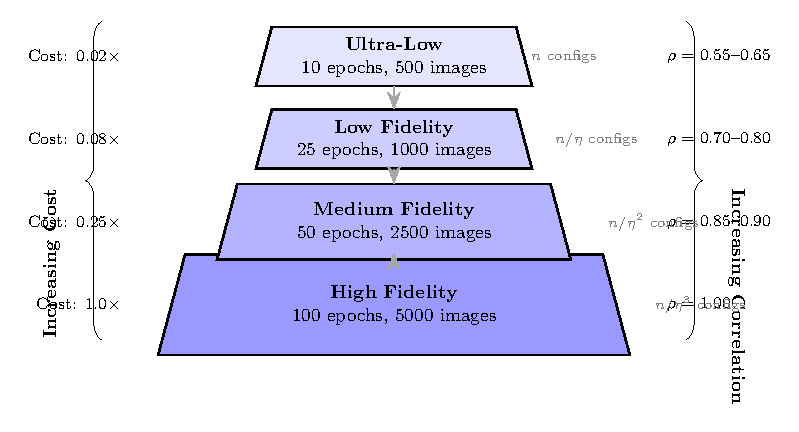
\includegraphics[width=0.85\textwidth]{figures/ch08_fig1_fidelity_pyramid.pdf}
\caption{Multi-fidelity evaluation pyramid showing the cost-correlation tradeoff across fidelity levels. Lower fidelity levels (top) evaluate many configurations at low cost but with reduced correlation to full-fidelity performance. Higher fidelity levels (bottom) provide accurate performance estimates but at substantially greater computational expense. The progressive filtering strategy evaluates $n$ configurations at ultra-low fidelity, promoting only the top $1/\eta$ fraction to each subsequent level.}
\label{fig:fidelity_pyramid}
\end{figure}

\subsection{Correlation Between Fidelity Levels}

The effectiveness of multi-fidelity optimization depends critically on the correlation structure between low-fidelity and high-fidelity evaluations. Let $\rho(r_1, r_2)$ denote the Spearman rank correlation between configuration rankings at fidelity levels $r_1$ and $r_2$. Effective multi-fidelity optimization requires $\rho(r_{\text{low}}, r_{\text{high}}) > 0.5$ to ensure that low-fidelity evaluations provide meaningful guidance for configuration selection.

Empirical studies of neural network hyperparameter optimization have demonstrated that early-epoch performance correlates strongly with final performance for many architecture and optimization configurations. This correlation arises from the learning dynamics of stochastic gradient descent, where configurations that learn rapidly in early epochs tend to maintain their relative advantage through continued training. However, pathological cases exist where early performance inversely correlates with final performance, particularly for configurations with aggressive learning rates that achieve rapid initial progress but subsequently diverge.

The dataset size dimension exhibits more complex correlation behavior. Reducing dataset size increases the variance of learned models due to reduced coverage of the underlying data distribution, potentially causing rank reversals between configurations. The impact is particularly pronounced for synthetic data optimization, where dataset diversity directly influences the model's ability to generalize to real-world data. Configurations that perform well on small synthetic datasets may fail to transfer effectively when scaled to larger training sets if they exploit spurious correlations in the limited data.

\subsection{Optimal Fidelity Scheduling}

The allocation of computational budget across fidelity levels represents a critical design decision in multi-fidelity optimization. Aggressive use of low-fidelity evaluations maximizes the number of configurations explored but risks discarding promising configurations due to noisy low-fidelity estimates. Conservative strategies that emphasize high-fidelity evaluations provide more reliable performance estimates but explore fewer configurations within a fixed budget.

Theoretical analysis of multi-fidelity Bayesian optimization suggests that optimal budget allocation depends on the cost ratio between fidelity levels and the correlation structure of the objective function. When low-fidelity evaluations are substantially cheaper than high-fidelity evaluations and exhibit strong correlation, aggressive allocation to low-fidelity exploration followed by selective high-fidelity validation maximizes expected optimization performance. The successive halving and Hyperband algorithms, developed in subsequent sections, provide principled approaches to this allocation problem.

% TikZ diagram for multi-fidelity evaluation flow
\begin{figure}[htbp]
\centering
\begin{tikzpicture}[
    node distance=1.5cm,
    box/.style={rectangle, draw, rounded corners, minimum width=2.5cm, minimum height=0.8cm, align=center, fill=blue!10},
    decision/.style={diamond, draw, aspect=2, minimum width=2cm, fill=yellow!20},
    arrow/.style={->, >=stealth, thick}
]
    % Nodes
    \node[box] (sample) {Sample\\Configuration $\theta$};
    \node[box, below=of sample] (lowfid) {Low-Fidelity\\Evaluation};
    \node[decision, below=of lowfid] (promote1) {Top\\$1/\eta$?};
    \node[box, below=of promote1] (medfid) {Medium-Fidelity\\Evaluation};
    \node[decision, below=of medfid] (promote2) {Top\\$1/\eta$?};
    \node[box, below=of promote2] (highfid) {High-Fidelity\\Evaluation};
    \node[box, right=3cm of promote1] (discard1) {Discard\\Configuration};
    \node[box, right=3cm of promote2] (discard2) {Discard\\Configuration};

    % Arrows
    \draw[arrow] (sample) -- (lowfid);
    \draw[arrow] (lowfid) -- (promote1);
    \draw[arrow] (promote1) -- node[left] {Yes} (medfid);
    \draw[arrow] (promote1) -- node[above] {No} (discard1);
    \draw[arrow] (medfid) -- (promote2);
    \draw[arrow] (promote2) -- node[left] {Yes} (highfid);
    \draw[arrow] (promote2) -- node[above] {No} (discard2);

    % Labels
    \node[left=0.5cm of lowfid, align=right] {Cost: $c_{\min}$\\Configs: $n$};
    \node[left=0.5cm of medfid, align=right] {Cost: $\eta \cdot c_{\min}$\\Configs: $n/\eta$};
    \node[left=0.5cm of highfid, align=right] {Cost: $\eta^2 \cdot c_{\min}$\\Configs: $n/\eta^2$};
\end{tikzpicture}
\caption{Multi-fidelity evaluation flow with progressive resource allocation. Configurations are evaluated at increasing fidelity levels, with only the top $1/\eta$ fraction promoted at each stage. This structure enables exploration of many configurations while concentrating computational resources on the most promising candidates.}
\label{fig:multi_fidelity_flow}
\end{figure}

\section{Successive Halving Algorithm}
\label{sec:successive_halving}

Successive halving provides a principled approach to multi-fidelity hyperparameter optimization by iteratively eliminating the worst-performing configurations while increasing the resource allocation to survivors. The algorithm achieves provable efficiency gains over uniform allocation strategies when low-fidelity evaluations correlate with high-fidelity performance.

\subsection{Mathematical Foundation}

Consider the problem of identifying the best configuration from a set of $n$ candidates, where each configuration $\theta_i$ has unknown quality $f(\theta_i)$ that can only be observed through noisy evaluations at varying fidelity levels. The successive halving algorithm operates under a total budget constraint $B$ and seeks to maximize the probability of correctly identifying the best configuration.

Let $r_{\min}$ denote the minimum resource allocation per configuration and $r_{\max}$ the maximum allocation required for reliable evaluation. The algorithm proceeds in $K = \lfloor \log_\eta(r_{\max}/r_{\min}) \rfloor$ rounds, where $\eta > 1$ is the elimination rate. At each round $k$, the algorithm evaluates remaining configurations with resource allocation $r_k = r_{\min} \cdot \eta^k$ and eliminates the bottom $(1 - 1/\eta)$ fraction based on observed performance.

The total resource consumption of successive halving can be bounded as:

\begin{equation}
B_{\text{SH}} = \sum_{k=0}^{K} n_k \cdot r_k = \sum_{k=0}^{K} \frac{n}{\eta^k} \cdot r_{\min} \cdot \eta^k = (K+1) \cdot n \cdot r_{\min}
\label{eq:sh_budget}
\end{equation}

where $n_k = n/\eta^k$ denotes the number of configurations remaining at round $k$. This budget scales linearly with the initial number of configurations and logarithmically with the fidelity range $r_{\max}/r_{\min}$, enabling exploration of large configuration spaces within modest computational budgets.

\subsection{Algorithm Description}

The successive halving algorithm proceeds through a sequence of elimination rounds, progressively focusing computational resources on promising configurations while discarding those exhibiting poor early performance. Algorithm~\ref{alg:successive_halving} presents the complete procedure.

\begin{algorithm}[htbp]
\caption{Successive Halving for Multi-Fidelity Optimization}
\label{alg:successive_halving}
\begin{algorithmic}[1]
\Require Configuration space $\Theta$, number of configurations $n$, minimum resource $r_{\min}$, maximum resource $r_{\max}$, elimination rate $\eta$
\Ensure Best configuration $\theta^*$
\State $K \gets \lfloor \log_\eta(r_{\max}/r_{\min}) \rfloor$ \Comment{Number of rounds}
\State $S_0 \gets \text{SampleConfigurations}(\Theta, n)$ \Comment{Initial configuration set}
\For{$k = 0, 1, \ldots, K$}
    \State $r_k \gets r_{\min} \cdot \eta^k$ \Comment{Resource allocation for round $k$}
    \State $n_k \gets |S_k|$ \Comment{Number of surviving configurations}
    \For{each $\theta \in S_k$}
        \State $v_\theta \gets \text{Evaluate}(\theta, r_k)$ \Comment{Evaluate at current fidelity}
    \EndFor
    \State $S_{k+1} \gets \text{TopFraction}(S_k, 1/\eta, \{v_\theta\})$ \Comment{Keep top $1/\eta$ fraction}
\EndFor
\State $\theta^* \gets \arg\max_{\theta \in S_K} v_\theta$ \Comment{Return best configuration}
\State \Return $\theta^*$
\end{algorithmic}
\end{algorithm}

The \textsc{SampleConfigurations} procedure generates initial configurations through random sampling or quasi-random sequences such as Sobol or Halton. The \textsc{Evaluate} function executes the synthetic data optimization pipeline with the specified configuration and resource allocation, returning the observed performance metric. The \textsc{TopFraction} procedure sorts configurations by observed performance and retains only the top $1/\eta$ fraction for subsequent rounds.

\subsection{Bracket Configuration}

The successive halving algorithm requires specification of four primary hyperparameters that collectively determine its behavior. The initial configuration count $n$ controls the breadth of exploration, with larger values enabling evaluation of more diverse configurations at the cost of reduced per-configuration resources. The elimination rate $\eta$ determines the aggressiveness of pruning, with typical values ranging from 2 to 4. Smaller values of $\eta$ result in more gradual elimination but require additional rounds, while larger values enable faster convergence at the risk of prematurely discarding good configurations.

The minimum and maximum resource allocations $r_{\min}$ and $r_{\max}$ define the fidelity range over which the algorithm operates. The minimum allocation should be chosen to provide sufficient signal for meaningful configuration comparison while minimizing computational cost. For synthetic data optimization with YOLO, empirical evidence suggests $r_{\min}$ corresponding to 10-25 training epochs on 500-1,000 images provides adequate discrimination between configurations.

\subsection{Resource Allocation Analysis}

The resource allocation strategy of successive halving exhibits favorable theoretical properties when the objective function satisfies certain regularity conditions. Under the assumption that low-fidelity rankings correlate perfectly with high-fidelity rankings, successive halving identifies the optimal configuration with probability 1 while consuming resources logarithmic in the number of initial configurations.

More realistic analysis accounts for rank correlation degradation at low fidelities. Let $\epsilon$ denote the probability that a configuration's rank changes by more than $1/\eta$ fraction between adjacent fidelity levels. The success probability of successive halving degrades gracefully with $\epsilon$, maintaining high accuracy when $\epsilon < 1/\eta$. This analysis motivates the choice of conservative elimination rates in settings where low-fidelity correlation is uncertain.

% TikZ diagram for successive halving bracket structure
\begin{figure}[htbp]
\centering
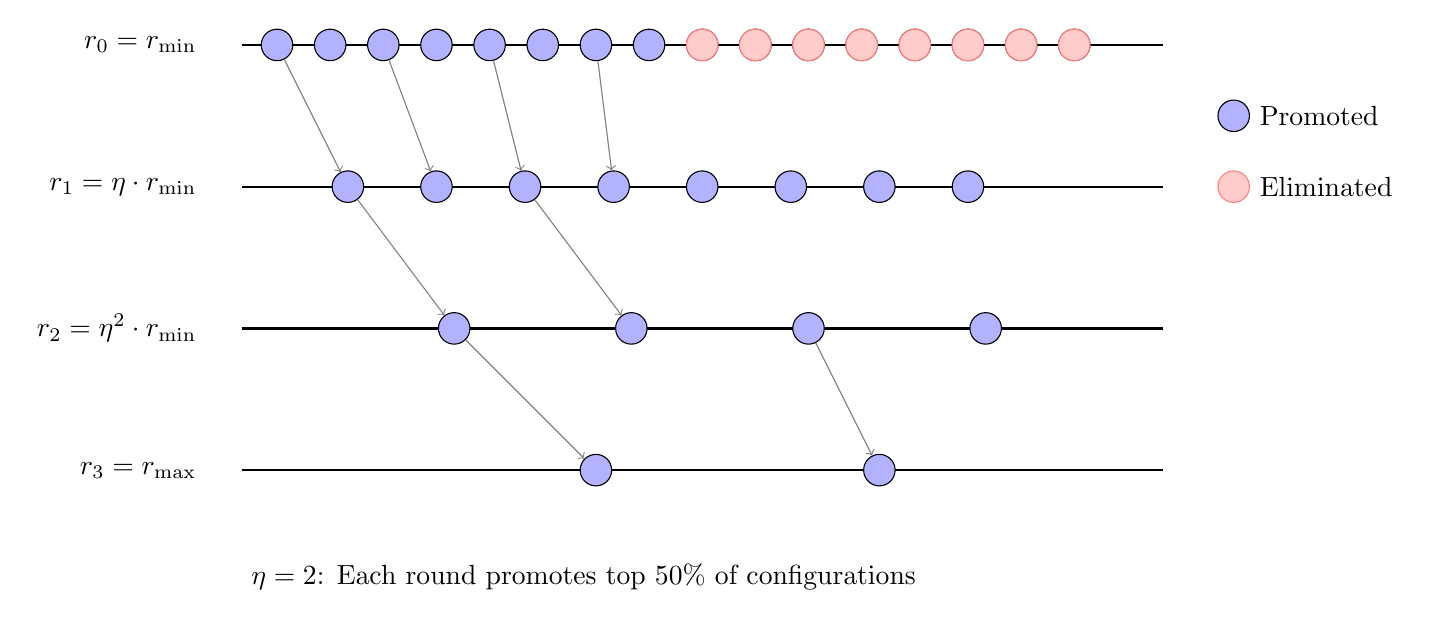
\begin{tikzpicture}[
    scale=0.9,
    config/.style={circle, draw, minimum size=0.4cm, inner sep=0, fill=blue!30},
    eliminated/.style={circle, draw, minimum size=0.4cm, inner sep=0, fill=red!20, draw=red!50},
    rung/.style={thick}
]
    % Rung labels
    \node[anchor=east] at (-0.5, 0) {$r_0 = r_{\min}$};
    \node[anchor=east] at (-0.5, -2) {$r_1 = \eta \cdot r_{\min}$};
    \node[anchor=east] at (-0.5, -4) {$r_2 = \eta^2 \cdot r_{\min}$};
    \node[anchor=east] at (-0.5, -6) {$r_3 = r_{\max}$};

    % Rung lines
    \draw[rung] (0, 0) -- (13, 0);
    \draw[rung] (0, -2) -- (13, -2);
    \draw[rung] (0, -4) -- (13, -4);
    \draw[rung] (0, -6) -- (13, -6);

    % Round 0: 16 configurations
    \foreach \i in {1,...,16} {
        \pgfmathsetmacro{\x}{0.5 + (\i-1)*0.75}
        \node[config] (r0c\i) at (\x, 0) {};
    }

    % Round 1: 8 configurations (top half promoted)
    \foreach \i in {1,...,8} {
        \pgfmathsetmacro{\x}{1.5 + (\i-1)*1.25}
        \node[config] (r1c\i) at (\x, -2) {};
    }
    % Eliminated in round 0
    \foreach \i in {9,...,16} {
        \pgfmathsetmacro{\x}{0.5 + (\i-1)*0.75}
        \node[eliminated] at (\x, 0) {};
    }

    % Round 2: 4 configurations
    \foreach \i in {1,...,4} {
        \pgfmathsetmacro{\x}{3 + (\i-1)*2.5}
        \node[config] (r2c\i) at (\x, -4) {};
    }

    % Round 3: 2 configurations
    \foreach \i in {1,...,2} {
        \pgfmathsetmacro{\x}{5 + (\i-1)*4}
        \node[config] (r3c\i) at (\x, -6) {};
    }

    % Connection lines (sample)
    \draw[->, gray] (r0c1) -- (r1c1);
    \draw[->, gray] (r0c3) -- (r1c2);
    \draw[->, gray] (r0c5) -- (r1c3);
    \draw[->, gray] (r0c7) -- (r1c4);
    \draw[->, gray] (r1c1) -- (r2c1);
    \draw[->, gray] (r1c3) -- (r2c2);
    \draw[->, gray] (r2c1) -- (r3c1);
    \draw[->, gray] (r2c3) -- (r3c2);

    % Legend
    \node[config, label=right:Promoted] at (14, -1) {};
    \node[eliminated, label=right:Eliminated] at (14, -2) {};

    % Annotation
    \node[anchor=west, align=left] at (0, -7.5) {$\eta = 2$: Each round promotes top 50\% of configurations};
\end{tikzpicture}
\caption{Successive halving bracket structure with $n=16$ initial configurations and elimination rate $\eta=2$. Blue nodes represent configurations promoted to the next fidelity level, while red nodes indicate eliminated configurations. The algorithm requires $\log_\eta(n) = 4$ rounds to identify the final winner.}
\label{fig:sh_bracket}
\end{figure}

\section{Hyperband}
\label{sec:hyperband}

While successive halving provides an effective multi-fidelity optimization strategy, its performance depends critically on the choice of initial configuration count $n$. Choosing $n$ too small limits exploration of the configuration space, while choosing $n$ too large spreads resources thinly across initial low-fidelity evaluations. The Hyperband algorithm addresses this tradeoff by running multiple successive halving brackets with different initial configuration counts, automatically adapting to the unknown exploration-exploitation tradeoff.

\subsection{Extension of Successive Halving}

Hyperband operates by executing $s_{\max} + 1$ successive halving brackets in sequence, where each bracket $s \in \{0, 1, \ldots, s_{\max}\}$ uses a different initial configuration count and minimum resource allocation. The parameter $s_{\max} = \lfloor \log_\eta(r_{\max}/r_{\min}) \rfloor$ equals the maximum number of halving rounds possible within the fidelity range.

For bracket $s$, the algorithm initializes $n_s = \lceil (s_{\max}+1) \eta^s / (s+1) \rceil$ configurations with minimum resource allocation $r_s = r_{\max} \eta^{-s}$. This allocation scheme ensures that each bracket consumes approximately equal total resources while exploring different regions of the exploration-exploitation spectrum. Brackets with larger $s$ values explore more configurations at lower initial fidelities, while brackets with smaller $s$ values explore fewer configurations but provide each with higher initial resources.

\subsection{Multiple Bracket Strategy}

The multiple bracket strategy of Hyperband provides robustness to uncertainty about the optimal exploration-exploitation tradeoff. When low-fidelity evaluations strongly predict high-fidelity performance, brackets with large $s$ values (aggressive exploration) dominate performance by efficiently screening many configurations. When low-fidelity predictions are unreliable, brackets with small $s$ values (conservative exploration) succeed by providing configurations with sufficient resources for reliable evaluation.

The total resource consumption of a complete Hyperband iteration, executing all $s_{\max}+1$ brackets, can be bounded as:

\begin{equation}
B_{\text{HB}} \leq (s_{\max}+1)^2 \cdot r_{\max}
\label{eq:hb_budget}
\end{equation}

This resource consumption scales quadratically with the logarithm of the fidelity range, maintaining efficiency for large fidelity ranges while providing comprehensive coverage of the exploration-exploitation spectrum.

\subsection{Theoretical Guarantees}

Hyperband provides theoretical guarantees on optimization performance under mild regularity assumptions. Let $\nu$ denote the fraction of configurations with quality within $\epsilon$ of optimal. Under the assumption that low-fidelity rankings preserve the relative ordering of near-optimal configurations, Hyperband identifies an $\epsilon$-optimal configuration with high probability using resources:

\begin{equation}
B^* = O\left( \frac{r_{\max}}{\nu} \log\left(\frac{1}{\nu}\right) \log\left(\frac{r_{\max}}{r_{\min}}\right) \right)
\label{eq:hb_guarantee}
\end{equation}

This guarantee improves upon uniform random search, which requires $O(r_{\max}/\nu)$ resources, by a factor logarithmic in the fidelity range. The improvement becomes substantial when the fidelity range spans multiple orders of magnitude, as is typical in neural network training settings.

\subsection{Comparison with Pure Bayesian Optimization}

Pure Bayesian optimization constructs a probabilistic surrogate model of the objective function and uses this model to guide sequential configuration selection through an acquisition function. While Bayesian optimization achieves strong theoretical and empirical performance in low-dimensional continuous optimization, its advantages diminish in the multi-fidelity setting for several reasons.

First, Gaussian process surrogate models incur computational costs that scale cubically with the number of observations, limiting their applicability when hundreds or thousands of low-fidelity evaluations are collected. Second, extending Bayesian optimization to the multi-fidelity setting requires modeling the correlation structure between fidelity levels, introducing additional complexity and potential for model misspecification. Third, the sequential nature of Bayesian optimization limits parallelization opportunities, while successive halving and Hyperband naturally support parallel evaluation within each round.

Empirical comparisons across hyperparameter optimization benchmarks demonstrate that Hyperband matches or exceeds the performance of Gaussian process-based Bayesian optimization while providing substantially faster wall-clock convergence through parallelization. The BOHB algorithm, developed in the following section, combines the strengths of both approaches by using Bayesian optimization for configuration sampling within the Hyperband framework.

Figure~\ref{fig:hyperband_brackets} illustrates the complete bracket structure of Hyperband, showing how different brackets explore the configuration space with varying levels of aggressiveness.

\begin{figure}[htbp]
\centering
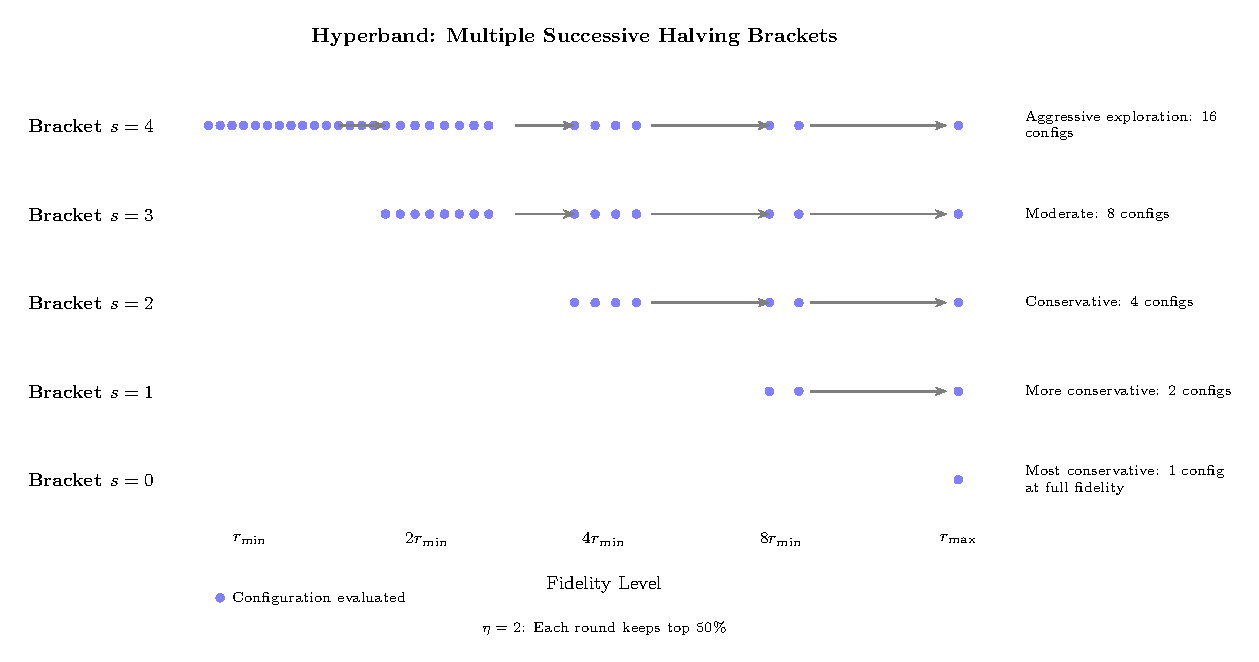
\includegraphics[width=0.95\textwidth]{figures/ch08_fig2_hyperband_brackets.pdf}
\caption{Hyperband bracket structure with $\eta = 2$ and $s_{\max} = 4$. Each row represents a different bracket with varying exploration-exploitation tradeoffs. Bracket $s=4$ (top) explores 16 configurations starting at minimum fidelity, aggressively filtering through successive halving. Bracket $s=0$ (bottom) evaluates a single configuration at maximum fidelity. The multiple bracket strategy provides robustness to uncertainty about optimal allocation between exploration and exploitation.}
\label{fig:hyperband_brackets}
\end{figure}

\begin{algorithm}[htbp]
\caption{Hyperband Algorithm}
\label{alg:hyperband}
\begin{algorithmic}[1]
\Require Configuration space $\Theta$, minimum resource $r_{\min}$, maximum resource $r_{\max}$, elimination rate $\eta$
\Ensure Best configuration $\theta^*$
\State $s_{\max} \gets \lfloor \log_\eta(r_{\max}/r_{\min}) \rfloor$
\State $B \gets (s_{\max} + 1) \cdot r_{\max}$ \Comment{Budget per Hyperband iteration}
\State $\theta^* \gets \text{null}$, $v^* \gets -\infty$
\For{$s = s_{\max}, s_{\max}-1, \ldots, 0$} \Comment{Outer loop over brackets}
    \State $n_s \gets \lceil \frac{B}{r_{\max}} \cdot \frac{\eta^s}{s+1} \rceil$ \Comment{Initial configurations for bracket $s$}
    \State $r_s \gets r_{\max} \cdot \eta^{-s}$ \Comment{Initial resource for bracket $s$}
    \State $S \gets \text{SampleConfigurations}(\Theta, n_s)$
    \For{$k = 0, 1, \ldots, s$} \Comment{Inner loop: successive halving}
        \State $n_k \gets \lfloor n_s \cdot \eta^{-k} \rfloor$
        \State $r_k \gets r_s \cdot \eta^k$
        \For{each $\theta \in S$}
            \State $v_\theta \gets \text{Evaluate}(\theta, r_k)$
            \If{$v_\theta > v^*$}
                \State $\theta^* \gets \theta$, $v^* \gets v_\theta$
            \EndIf
        \EndFor
        \State $S \gets \text{TopFraction}(S, 1/\eta, \{v_\theta\})$
    \EndFor
\EndFor
\State \Return $\theta^*$
\end{algorithmic}
\end{algorithm}

\section{BOHB: Combining Bayesian Optimization with Hyperband}
\label{sec:bohb}

The BOHB algorithm represents a sophisticated synthesis of Bayesian optimization and Hyperband that inherits the strengths of both approaches. By replacing the random configuration sampling of Hyperband with model-based sampling, BOHB achieves improved sample efficiency while maintaining the robustness and parallelization capabilities of the Hyperband framework.

\subsection{TPE Sampler Integration}

BOHB employs the Tree-structured Parzen Estimator as its surrogate model for configuration sampling. Unlike Gaussian process-based Bayesian optimization, which models the objective function directly, TPE models the conditional probability of configurations given their performance. Specifically, TPE maintains two density estimates: $\ell(\theta)$ modeling the density of configurations with performance above a threshold $\gamma$, and $g(\theta)$ modeling configurations below the threshold.

The acquisition function for TPE sampling takes the form:

\begin{equation}
\alpha(\theta) = \frac{\ell(\theta)}{g(\theta)}
\label{eq:tpe_acquisition}
\end{equation}

This ratio-based acquisition function naturally trades off exploration and exploitation by favoring configurations that are likely under the good-performance model $\ell(\theta)$ while unlikely under the poor-performance model $g(\theta)$. New configurations are sampled by drawing candidates from $\ell(\theta)$ and selecting those with highest acquisition values.

The computational efficiency of TPE derives from its kernel density estimation approach, which scales linearly with the number of observations rather than cubically as with Gaussian processes. This efficiency enables BOHB to effectively utilize the large number of low-fidelity observations generated by Hyperband's multiple brackets.

\subsection{Warm-Starting Strategies}

BOHB incorporates several warm-starting strategies to accelerate optimization by leveraging historical evaluation data. When optimizing a new synthetic data generation task, BOHB can initialize its TPE models using observations from related tasks, providing an informative prior that guides early exploration toward promising regions of the configuration space.

The multi-fidelity structure of BOHB enables sophisticated warm-starting through fidelity-conditional modeling. Observations from low-fidelity evaluations update the TPE models with appropriate weighting, providing dense coverage of the configuration space while allowing high-fidelity observations to dominate near-optimal configurations. This hierarchical modeling approach enables BOHB to efficiently allocate limited high-fidelity observations while maintaining comprehensive exploration through low-fidelity evaluations.

\subsection{Implementation with Optuna}

The Optuna hyperparameter optimization framework provides a production-ready implementation of BOHB that integrates seamlessly with Python-based machine learning workflows. Optuna's define-by-run API enables flexible specification of configuration spaces, including conditional parameters and hierarchical structures that frequently arise in synthetic data generation pipelines.

The following code fragment illustrates the integration of BOHB with Optuna for synthetic data optimization:

\begin{verbatim}
import optuna
from optuna.pruners import HyperbandPruner
from optuna.samplers import TPESampler

def objective(trial):
    # Define synthetic data parameters
    brightness_range = trial.suggest_float("brightness", 0.5, 1.5)
    contrast_range = trial.suggest_float("contrast", 0.5, 1.5)
    noise_level = trial.suggest_float("noise", 0.0, 0.1)

    # Multi-fidelity: report intermediate values
    for epoch in [10, 25, 50, 100]:
        mAP = train_and_evaluate(brightness_range, contrast_range,
                                  noise_level, epochs=epoch)
        trial.report(mAP, epoch)
        if trial.should_prune():
            raise optuna.TrialPruned()

    return mAP

study = optuna.create_study(
    direction="maximize",
    sampler=TPESampler(n_startup_trials=10),
    pruner=HyperbandPruner(min_resource=10, max_resource=100,
                           reduction_factor=3)
)
study.optimize(objective, n_trials=100)
\end{verbatim}

\subsection{Complete BOHB Algorithm}

Algorithm~\ref{alg:bohb} presents the complete BOHB procedure, integrating TPE-based configuration sampling with the Hyperband bracket structure.

\begin{algorithm}[htbp]
\caption{BOHB: Bayesian Optimization with Hyperband}
\label{alg:bohb}
\begin{algorithmic}[1]
\Require Configuration space $\Theta$, resource bounds $r_{\min}, r_{\max}$, elimination rate $\eta$, TPE quantile $\gamma$
\Ensure Best configuration $\theta^*$
\State $s_{\max} \gets \lfloor \log_\eta(r_{\max}/r_{\min}) \rfloor$
\State Initialize TPE models $\mathcal{M}_r$ for each fidelity level $r$
\State $\mathcal{D} \gets \emptyset$ \Comment{Observation history}
\State $\theta^* \gets \text{null}$, $v^* \gets -\infty$
\While{budget not exhausted}
    \For{$s = s_{\max}, s_{\max}-1, \ldots, 0$}
        \State $n_s \gets \lceil \frac{(s_{\max}+1) \eta^s}{s+1} \rceil$
        \State $r_s \gets r_{\max} \cdot \eta^{-s}$
        \State $S \gets \emptyset$
        \For{$i = 1, \ldots, n_s$}
            \If{$|\mathcal{D}| < n_{\text{startup}}$}
                \State $\theta \gets \text{RandomSample}(\Theta)$
            \Else
                \State $\theta \gets \text{TPESample}(\Theta, \mathcal{M}_{r_s}, \gamma)$
            \EndIf
            \State $S \gets S \cup \{\theta\}$
        \EndFor
        \For{$k = 0, 1, \ldots, s$}
            \State $r_k \gets r_s \cdot \eta^k$
            \For{each $\theta \in S$}
                \State $v_\theta \gets \text{Evaluate}(\theta, r_k)$
                \State $\mathcal{D} \gets \mathcal{D} \cup \{(\theta, r_k, v_\theta)\}$
                \State Update TPE model $\mathcal{M}_{r_k}$ with new observation
                \If{$r_k = r_{\max}$ and $v_\theta > v^*$}
                    \State $\theta^* \gets \theta$, $v^* \gets v_\theta$
                \EndIf
            \EndFor
            \State $S \gets \text{TopFraction}(S, 1/\eta, \{v_\theta\})$
        \EndFor
    \EndFor
\EndWhile
\State \Return $\theta^*$
\end{algorithmic}
\end{algorithm}

\section{Budget Allocation Strategy}
\label{sec:budget_allocation}

Effective utilization of limited computational resources requires careful planning of budget allocation across optimization phases. This section develops a comprehensive framework for budget planning in synthetic data optimization projects, providing concrete recommendations based on empirical observations and theoretical analysis.

\subsection{Recommended Phase Breakdown}

The optimization process naturally decomposes into three phases with distinct objectives and resource requirements. The exploration phase seeks to identify promising regions of the configuration space through broad, low-fidelity evaluation. The refinement phase narrows the search within identified promising regions using medium-fidelity evaluations. The validation phase provides high-confidence performance estimates for final configuration selection through full-fidelity evaluation.

Table~\ref{tab:phase_breakdown} presents recommended budget allocations for each phase under varying total budget constraints.

\begin{table}[htbp]
\centering
\caption{Recommended Budget Allocation by Optimization Phase}
\label{tab:phase_breakdown}
\begin{tabular}{lccc}
\hline
\textbf{Phase} & \textbf{Budget Share} & \textbf{Fidelity Level} & \textbf{Objective} \\
\hline
Exploration & 35--45\% & Low (10--25 epochs) & Identify promising regions \\
Refinement & 30--40\% & Medium (25--50 epochs) & Narrow candidate set \\
Validation & 20--30\% & High (100 epochs) & Final selection \\
\hline
\end{tabular}
\end{table}

The exploration phase consumes the largest budget fraction but at the lowest per-configuration cost, enabling evaluation of 50-200 diverse configurations. The refinement phase reduces the candidate set to 10-30 configurations while providing more reliable performance estimates. The validation phase concentrates resources on 5-15 finalist configurations to enable confident selection of the optimal configuration.

\subsection{Exploration vs. Validation Budget}

The allocation between exploration and validation phases represents a fundamental tradeoff in budget-constrained optimization. Allocating excessive budget to exploration maximizes configuration coverage but may fail to accurately rank top configurations due to limited high-fidelity evaluation. Conversely, allocating excessive budget to validation provides accurate rankings but only for a restricted set of configurations, risking exclusion of the global optimum.

Theoretical analysis suggests that optimal allocation depends on the shape of the configuration quality distribution. When good configurations are rare, exploration-heavy allocation increases the probability of encountering at least one good configuration. When good configurations are common, validation-heavy allocation maximizes the probability of correctly identifying the best among discovered configurations.

For synthetic data optimization, empirical evidence suggests that good configurations exist at moderate density in typical configuration spaces, supporting the balanced allocation in Table~\ref{tab:phase_breakdown}. Projects with highly constrained budgets should prioritize exploration to ensure sufficient configuration diversity, while projects with generous budgets can increase validation allocation to reduce selection uncertainty.

\subsection{Reserve Budget Considerations}

Practical optimization projects should maintain a reserve budget of 10-15\% of total resources to accommodate unexpected requirements. Common uses of reserve budget include extended evaluation of surprisingly good configurations discovered late in optimization, investigation of configuration sensitivity through replicated evaluations, and recovery from failed evaluations due to hardware or software issues.

The reserve budget also supports adaptive reallocation between phases based on intermediate results. If exploration reveals unexpectedly dense promising regions, reserve budget can fund additional refinement evaluations. Conversely, if promising configurations are sparse, reserve budget can extend the exploration phase.

\subsection{Total Resource Estimation Framework}

Table~\ref{tab:resource_estimation} provides a complete framework for estimating total resource requirements based on project parameters. The framework accounts for all cost components and provides confidence intervals reflecting uncertainty in individual evaluation costs.

\begin{table}[htbp]
\centering
\caption{Total Resource Estimation Framework for Synthetic Data Optimization}
\label{tab:resource_estimation}
\begin{tabular}{lccr}
\hline
\textbf{Phase} & \textbf{Configurations} & \textbf{Cost/Config (GPU-hr)} & \textbf{Phase Total} \\
\hline
Exploration (Low) & 100 & 0.3--0.5 & 30--50 GPU-hr \\
Refinement (Med) & 25 & 1.0--1.5 & 25--38 GPU-hr \\
Validation (High) & 10 & 3.0--4.0 & 30--40 GPU-hr \\
Reserve & -- & -- & 10--15 GPU-hr \\
\hline
\textbf{Total} & & & \textbf{95--143 GPU-hr} \\
\hline
\end{tabular}
\end{table}

This resource estimate assumes a dataset size of 5,000 images at full fidelity, 100 training epochs for high-fidelity evaluation, and a YOLO-medium architecture. Projects using larger datasets, longer training, or more complex architectures should scale estimates proportionally. Cloud computing costs at typical GPU rental rates of \$1-3 per GPU-hour translate this estimate to \$100-400 total project cost, demonstrating the economic feasibility of rigorous synthetic data optimization.

Figure~\ref{fig:budget_allocation} provides a visual summary of the three-phase budget allocation strategy and the configuration filtering funnel.

\begin{figure}[htbp]
\centering
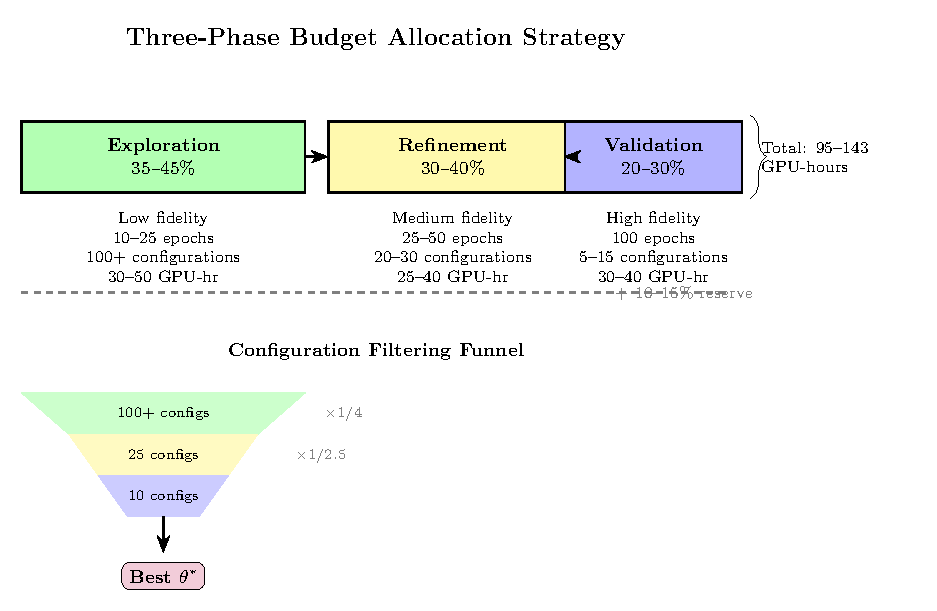
\includegraphics[width=0.9\textwidth]{figures/ch08_fig4_budget_allocation.pdf}
\caption{Three-phase budget allocation strategy for synthetic data optimization. The exploration phase (35--45\% of budget) evaluates 100+ configurations at low fidelity to identify promising regions. The refinement phase (30--40\%) narrows candidates to approximately 25 using medium-fidelity evaluation. The validation phase (20--30\%) provides high-confidence performance estimates for the 10 finalist configurations. A 10--15\% reserve accommodates unexpected requirements. The configuration filtering funnel (bottom) illustrates how progressive filtering concentrates resources on the most promising configurations.}
\label{fig:budget_allocation}
\end{figure}

\section{Convergence Detection}
\label{sec:convergence_detection}

Detecting convergence in black-box optimization is complicated by the inherent noise in objective function evaluations and the absence of gradient information. This section develops principled methods for convergence detection that enable early termination when further optimization is unlikely to yield meaningful improvement, conserving computational resources for subsequent experiments.

\subsection{Detecting Convergence in Noisy Settings}

The synthetic data optimization objective exhibits substantial evaluation noise arising from stochastic initialization, random sampling during training, and the inherent variability of performance metrics on finite validation sets. This noise complicates convergence detection by obscuring the underlying optimization trajectory.

Formal convergence in stochastic optimization is typically defined in terms of the distance to a stationary point of the expected objective. However, the black-box setting precludes computation of gradients or Hessians, necessitating convergence criteria based solely on observed objective values. A practical definition considers the optimization converged when the expected improvement from additional evaluations falls below a problem-specific threshold $\epsilon$.

Let $y_t^*$ denote the best observed objective value after $t$ evaluations. The optimization exhibits diminishing returns when:

\begin{equation}
\mathbb{E}[y_{t+\Delta}^* - y_t^* | \mathcal{D}_t] < \epsilon
\label{eq:convergence_criterion}
\end{equation}

where $\mathcal{D}_t$ represents the evaluation history and $\Delta$ denotes a lookahead horizon. Estimating this expectation requires modeling the objective function, which Bayesian optimization provides through its surrogate model.

\subsection{EMA-Based Stopping Criteria}

Exponential moving average filtering provides a robust approach to convergence detection that smooths noisy observations while maintaining sensitivity to recent improvements. Define the EMA of best observed values as:

\begin{equation}
\bar{y}_t = \alpha y_t^* + (1-\alpha) \bar{y}_{t-1}
\label{eq:ema_definition}
\end{equation}

where $\alpha \in (0, 1)$ controls the smoothing strength. The convergence criterion based on EMA improvement compares the current EMA to a lagged value:

\begin{equation}
\bar{y}_t - \bar{y}_{t-w} < \epsilon
\label{eq:ema_convergence}
\end{equation}

where $w$ is the lookback window size. This criterion triggers when the smoothed objective shows insufficient improvement over the lookback period.

The choice of smoothing parameter $\alpha$ and lookback window $w$ involves a tradeoff between responsiveness and robustness. Smaller $\alpha$ values (stronger smoothing) reduce false convergence detection due to noise but delay detection of true convergence. Typical values of $\alpha = 0.1$ to $0.3$ and $w = 10$ to $20$ evaluations provide good performance across optimization problems.

Figure~\ref{fig:convergence_detection} illustrates the convergence detection process, showing the relationship between raw observations, EMA smoothing, and convergence criteria.

\begin{figure}[htbp]
\centering
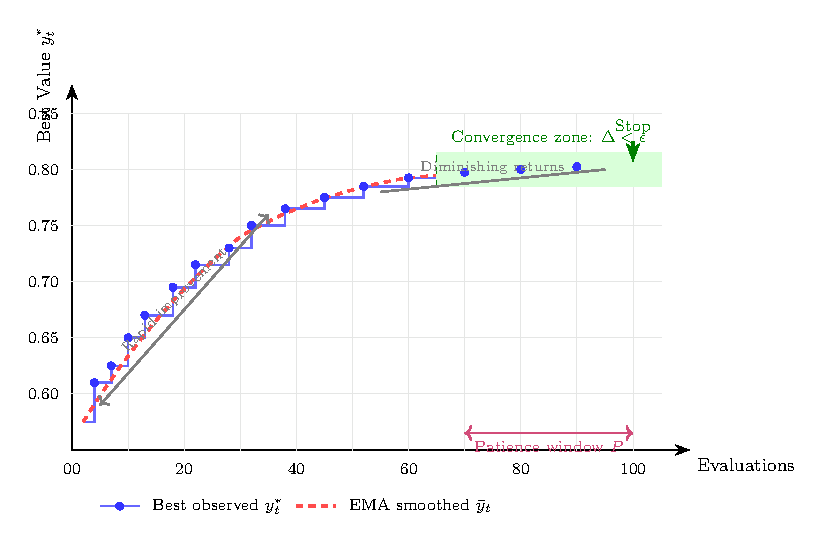
\includegraphics[width=0.85\textwidth]{figures/ch08_fig5_convergence_detection.pdf}
\caption{Convergence detection in sample-efficient optimization. The step function (solid blue) shows the best observed value $y_t^*$ over successive evaluations, with rapid improvement in early iterations followed by diminishing returns. The EMA-smoothed curve (dashed red) provides a noise-robust trajectory estimate. The convergence zone (green shaded region) indicates where improvement falls below threshold $\epsilon$. The patience window $P$ tracks evaluations without improvement, triggering termination when optimization has stagnated.}
\label{fig:convergence_detection}
\end{figure}

\subsection{Statistical Tests for Improvement}

Formal statistical testing provides rigorous convergence criteria with controlled false positive rates. The Mann-Whitney U test offers a nonparametric comparison between recent evaluations and historical evaluations, detecting whether recent observations come from a distribution with higher median.

Partition the evaluation history into recent observations $\{y_{t-w+1}, \ldots, y_t\}$ and historical observations $\{y_1, \ldots, y_{t-w}\}$. The null hypothesis $H_0$ asserts that recent observations are not stochastically greater than historical observations. Rejecting $H_0$ indicates continued improvement, while failing to reject suggests convergence.

The significance level $\alpha_{\text{test}}$ controls the false convergence rate, with typical values of 0.05 to 0.10 providing adequate sensitivity. When multiple statistical tests are performed across the optimization trajectory, appropriate corrections for multiple comparisons maintain the family-wise error rate.

\subsection{Patience-Based Early Stopping}

Patience-based stopping provides a simple yet effective convergence criterion that terminates optimization after a specified number of evaluations without improvement. Define the patience counter $p_t$ as:

\begin{equation}
p_t = \begin{cases}
0 & \text{if } y_t > y_{t-1}^* \\
p_{t-1} + 1 & \text{otherwise}
\end{cases}
\label{eq:patience_counter}
\end{equation}

The optimization terminates when $p_t$ exceeds the patience threshold $P$. This simple rule provides intuitive behavior while avoiding overfitting to noise when $P$ is chosen appropriately.

Algorithm~\ref{alg:convergence} presents a comprehensive convergence detection procedure that combines EMA-based, statistical, and patience-based criteria.

\begin{algorithm}[htbp]
\caption{Convergence Detection for Sample-Efficient Optimization}
\label{alg:convergence}
\begin{algorithmic}[1]
\Require Evaluation history $\mathcal{D} = \{(\theta_i, y_i)\}_{i=1}^t$, EMA parameter $\alpha$, lookback window $w$, improvement threshold $\epsilon$, patience $P$, significance level $\alpha_{\text{test}}$
\Ensure Convergence decision (Boolean)
\State Extract best values: $y_i^* = \max_{j \leq i} y_j$ for all $i$
\State \textit{// EMA-based criterion}
\State Compute EMA sequence: $\bar{y}_i = \alpha y_i^* + (1-\alpha)\bar{y}_{i-1}$
\State $\text{ema\_converged} \gets (\bar{y}_t - \bar{y}_{t-w} < \epsilon)$
\State \textit{// Patience-based criterion}
\State $p \gets 0$
\For{$i = 2, \ldots, t$}
    \If{$y_i^* > y_{i-1}^*$}
        \State $p \gets 0$
    \Else
        \State $p \gets p + 1$
    \EndIf
\EndFor
\State $\text{patience\_converged} \gets (p \geq P)$
\State \textit{// Statistical test criterion}
\State $U, p_{\text{val}} \gets \text{MannWhitneyU}(\{y_{t-w+1}, \ldots, y_t\}, \{y_1, \ldots, y_{t-w}\})$
\State $\text{stat\_converged} \gets (p_{\text{val}} > \alpha_{\text{test}})$
\State \textit{// Combined decision: require majority agreement}
\State $\text{votes} \gets \text{ema\_converged} + \text{patience\_converged} + \text{stat\_converged}$
\State \Return $(\text{votes} \geq 2)$
\end{algorithmic}
\end{algorithm}

\section{Parallelization and Efficiency}
\label{sec:parallelization}

Maximizing throughput in sample-efficient optimization requires effective utilization of available computational resources through parallelization. This section develops strategies for parallel evaluation that maintain the sample efficiency of sequential Bayesian optimization while exploiting multi-GPU environments.

\subsection{Batch Bayesian Optimization}

Batch Bayesian optimization extends the sequential framework to select multiple configurations for simultaneous evaluation. The key challenge lies in selecting a batch of configurations that collectively maximize information gain about the optimum, avoiding redundant evaluations of similar configurations.

The batch acquisition function extends the single-point acquisition to sets of configurations:

\begin{equation}
\alpha_B(S) = \mathbb{E}\left[ \max_{\theta \in S} \alpha(\theta) \mid S \text{ evaluated} \right]
\label{eq:batch_acquisition}
\end{equation}

Direct optimization of this batch acquisition function is computationally intractable for batch sizes greater than 2-3 configurations due to the combinatorial explosion of possible batches. Practical approaches employ greedy or quasi-greedy approximations that sequentially construct the batch while accounting for pending evaluations.

\subsection{Asynchronous Evaluation}

Asynchronous Bayesian optimization enables new configuration selection immediately when any evaluation completes, rather than waiting for all batch evaluations to finish. This approach maximizes GPU utilization by eliminating synchronization barriers and naturally handles heterogeneous evaluation times.

The asynchronous setting requires modeling pending evaluations that have been dispatched but not yet completed. A common approach imputes pending evaluations with their posterior mean under the current surrogate model, treating them as observed when selecting subsequent configurations. This hallucination strategy provides consistent surrogate predictions while avoiding duplicate selection of similar configurations.

\subsection{Local Penalization for Pending Points}

Local penalization provides an alternative approach to batch diversity that directly discourages selection of configurations near pending evaluations. The penalized acquisition function takes the form:

\begin{equation}
\alpha_P(\theta) = \alpha(\theta) \prod_{\theta' \in \mathcal{P}} \phi(\theta; \theta', L)
\label{eq:local_penalization}
\end{equation}

where $\mathcal{P}$ denotes the set of pending configurations and $\phi(\theta; \theta', L)$ is a penalty function that approaches zero as $\theta \to \theta'$ with characteristic length scale $L$. Common choices include Gaussian penalties $\phi(\theta; \theta', L) = 1 - \exp(-\|\theta - \theta'\|^2 / 2L^2)$ and hard exclusion regions.

The length scale $L$ should reflect the expected correlation range of the objective function. Setting $L$ too small permits redundant evaluations of nearly identical configurations, while setting $L$ too large unnecessarily restricts the search. Adaptive approaches estimate $L$ from the surrogate model's learned length scales, providing automatic calibration.

\subsection{GPU Utilization Strategies}

Maximizing GPU utilization in synthetic data optimization requires careful coordination of the generation, training, and evaluation pipeline stages. Several strategies improve utilization in multi-GPU environments.

Pipeline parallelism overlaps generation and training by beginning data generation for the next configuration while the current configuration trains. This overlap is particularly effective when generation time is comparable to training time, enabling near-100\% GPU utilization for the training-intensive portion of evaluation.

Data parallelism distributes training across multiple GPUs, reducing per-evaluation wall-clock time at the cost of increased per-evaluation GPU-hours. This tradeoff favors sequential throughput when wall-clock time is the limiting constraint, as in interactive optimization scenarios.

Configuration parallelism evaluates multiple configurations simultaneously on separate GPUs, maximizing throughput when sufficient configurations are available for parallel evaluation. This strategy integrates naturally with batch Bayesian optimization and asynchronous evaluation, providing the configurations needed to fully utilize available hardware.

Table~\ref{tab:parallelization} summarizes the tradeoffs between parallelization strategies for common hardware configurations.

\begin{table}[htbp]
\centering
\caption{GPU Parallelization Strategies and Their Characteristics}
\label{tab:parallelization}
\begin{tabular}{lccc}
\hline
\textbf{Strategy} & \textbf{GPUs} & \textbf{Throughput} & \textbf{Best When} \\
\hline
Sequential & 1 & 1$\times$ & Baseline \\
Pipeline & 1 & 1.3--1.5$\times$ & Gen time $\approx$ train time \\
Data parallel & 2--4 & 1.5--2$\times$ & Wall-clock constrained \\
Config parallel & 2--8 & 2--8$\times$ & GPU budget available \\
Hybrid & 4--8 & 3--6$\times$ & Balanced constraints \\
\hline
\end{tabular}
\end{table}

\section{Practical Implementation Considerations}
\label{sec:practical_implementation}

The translation of sample-efficient optimization algorithms from theory to practice requires attention to numerous implementation details that significantly impact performance and reliability. This section addresses common challenges and provides guidance for robust implementation.

\subsection{Handling Failed Evaluations}

The synthetic data optimization pipeline contains multiple potential failure points, including out-of-memory errors during training, numerical instabilities in loss computation, and I/O errors in data loading. Robust optimization frameworks must gracefully handle these failures without corrupting the evaluation history or biasing configuration selection.

Failed evaluations should be recorded with appropriate failure indicators rather than discarded, enabling analysis of failure patterns and informing future configuration selection. The surrogate model can incorporate failure information through censored observations or separate failure probability models, avoiding regions of the configuration space that consistently produce failures.

\subsection{Checkpointing and Resume}

Long-running optimization campaigns benefit from periodic checkpointing that enables resumption after interruptions. Checkpoint state should include the complete evaluation history, surrogate model parameters, random number generator state for reproducibility, and any accumulated statistics used for convergence detection.

When resuming from checkpoint, warm-starting the surrogate model with the recorded evaluation history enables immediate continuation without loss of accumulated information. For TPE-based methods, this warm-starting is straightforward as the model is reconstructed from observations. For Gaussian process methods, care must be taken to restore the exact model state including hyperparameter values.

\subsection{Reproducibility Considerations}

Reproducibility in sample-efficient optimization requires careful management of multiple sources of randomness. The configuration sampling process depends on random number generation, while the evaluation process depends on training randomness including initialization, data shuffling, and stochastic regularization.

For reproducibility, all random seeds should be recorded and associated with their corresponding evaluations. When comparing optimization algorithms or conducting ablation studies, shared random seeds for configuration sampling enable fair comparisons that isolate algorithmic differences from sampling variation.

\section{Summary}
\label{sec:ch8_summary}

This chapter has developed a comprehensive framework for sample-efficient optimization of synthetic data generation parameters, addressing the fundamental challenge of expensive black-box optimization under strict computational budgets. The multi-fidelity optimization paradigm enables efficient exploration of large configuration spaces by strategically allocating resources across evaluations of varying computational cost. The successive halving algorithm provides a principled approach to progressive elimination of unpromising configurations, while Hyperband extends this framework to automatically adapt to unknown exploration-exploitation tradeoffs.

The BOHB algorithm combines the strengths of Bayesian optimization and Hyperband, using model-based configuration sampling to improve upon random exploration while maintaining the robustness and parallelization capabilities of the Hyperband framework. Practical budget allocation strategies guide the distribution of computational resources across optimization phases, ensuring both adequate exploration and reliable validation of top configurations.

Convergence detection methods enable early termination when further optimization is unlikely to yield meaningful improvement, conserving resources for subsequent experiments. EMA-based smoothing, statistical testing, and patience-based criteria provide complementary perspectives on convergence that together enable robust detection in noisy settings. Parallelization strategies maximize throughput on multi-GPU systems through batch selection, asynchronous evaluation, and careful coordination of pipeline stages.

The techniques developed in this chapter collectively enable effective synthetic data optimization within practical computational budgets, transforming a problem that would require thousands of GPU-hours under naive approaches into one solvable with tens to hundreds of GPU-hours. This reduction in computational requirements makes rigorous optimization of synthetic data generation feasible for a broad range of research and industrial applications.

\end{chapter}
